\documentclass{beamer}
\usetheme{Madrid}
\usecolortheme{beaver}
\usepackage{color}
\usepackage{graphicx}
\usepackage[utf8]{inputenc}

\newcommand{\rs}[1]{{\color{red} RS:  #1}}

\newcommand{\bi}{\begin{itemize}}
\newcommand{\ei}{\end{itemize}}
\newcommand{\volk}{\text{Vol}_\text{K}}
\newcommand{\volcy}{\text{Vol}_\text{CY}}

%Information to be included in the title page:
\title[Hyperparameter Optimization]{String Theory meets Machine Learning\\
	- Hyperparameter Optimization}
\author{Robin Schneider}
\institute{Uppsala University}
\date{November 2020}


\begin{document}
	
\frame{\titlepage}

\begin{frame}
\frametitle{Performance}
How can we improve performance? \pause
\bi
\item Longer training time
\item More data
\item Data augmentation
\item Feature engineering
\item Changing architecture
\ei
\pause 
Changing all kinds of hyperparameters.
\end{frame}

\begin{frame}
\frametitle{(Hyper-)Parameters}
Here are some hyperparameters that influence the success of our experiments: \pause 
\bi
\item activation function
\item number of hidden units and layers
\item regularization parameters: l1, l2, dropout rate
\item learning rate, momentum, batch size 
\item kernel size, stride and padding
\item weight initialization
\ei
\pause Other parameters:
\bi
\item problem formulation
\item data used (e.g. ratio of train to val split, discarding of direct products)
\item seed (this might be bit controversial)
\item computational package (this too)
\ei
\end{frame}

\begin{frame}
\frametitle{Hyperparameter optimization}
How do we find the best values for our hyperparameters?
\pause 

Trial and error :(
\pause 
\bi
\item Human intuition
\item Grid Search
\item Random Search
\item Bayesian Optimization (GP, TPE)
\item Hyperband and BOHB
\item (Genetic Algorithms)
\ei
\end{frame}

\begin{frame}
\frametitle{CNNs and MNIST}
\begin{figure}[t]
	\begin{minipage}{0.5\linewidth}
		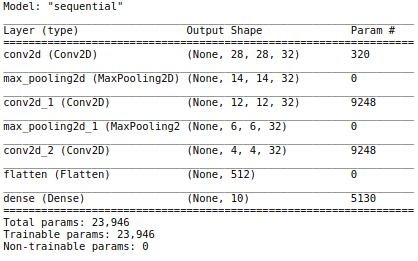
\includegraphics[scale=0.4]{mnist_cnn.png}
	\end{minipage}
	\begin{minipage}{0.45\linewidth}
		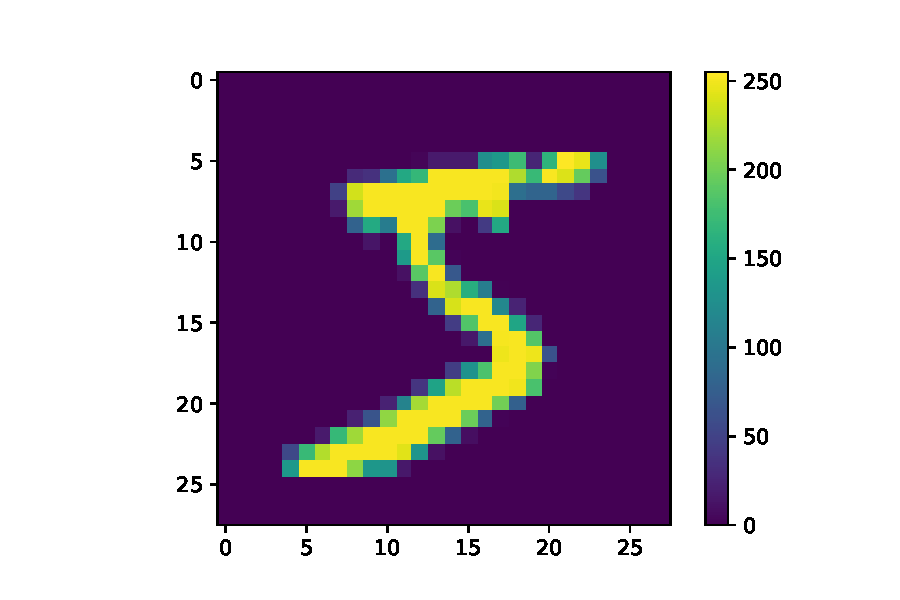
\includegraphics[scale=0.4]{mnist_digit.pdf}
	\end{minipage}
	%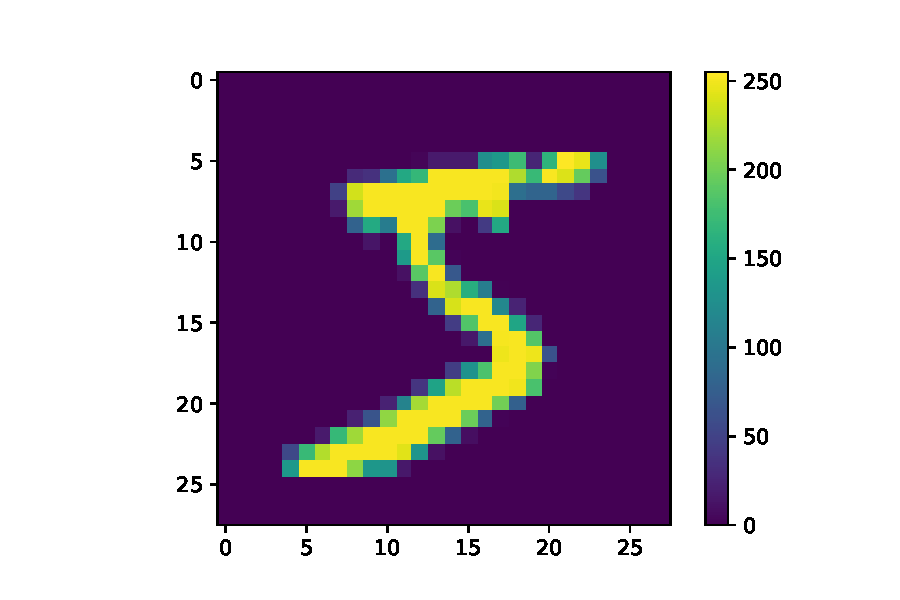
\includegraphics[scale=0.33]{mnist_digit.pdf}
	%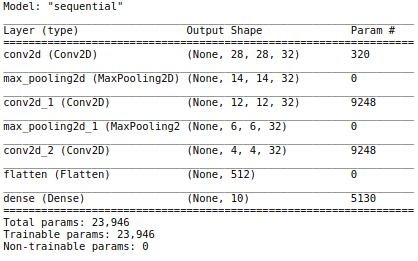
\includegraphics[scale=0.33]{mnist_cnn.png}
	\caption{\it Data sample of MNIST set and CNN to tackle the classification problem.}
	\label{fig:mnist}
\end{figure}
MNIST data set. (60.000, 10.000) train and test images. 28x28 with one color channel in the range of $\{0, ... , 255\}$.
\end{frame}

\begin{frame}
\frametitle{Grid Search}
\begin{figure}[t]
	\centering
	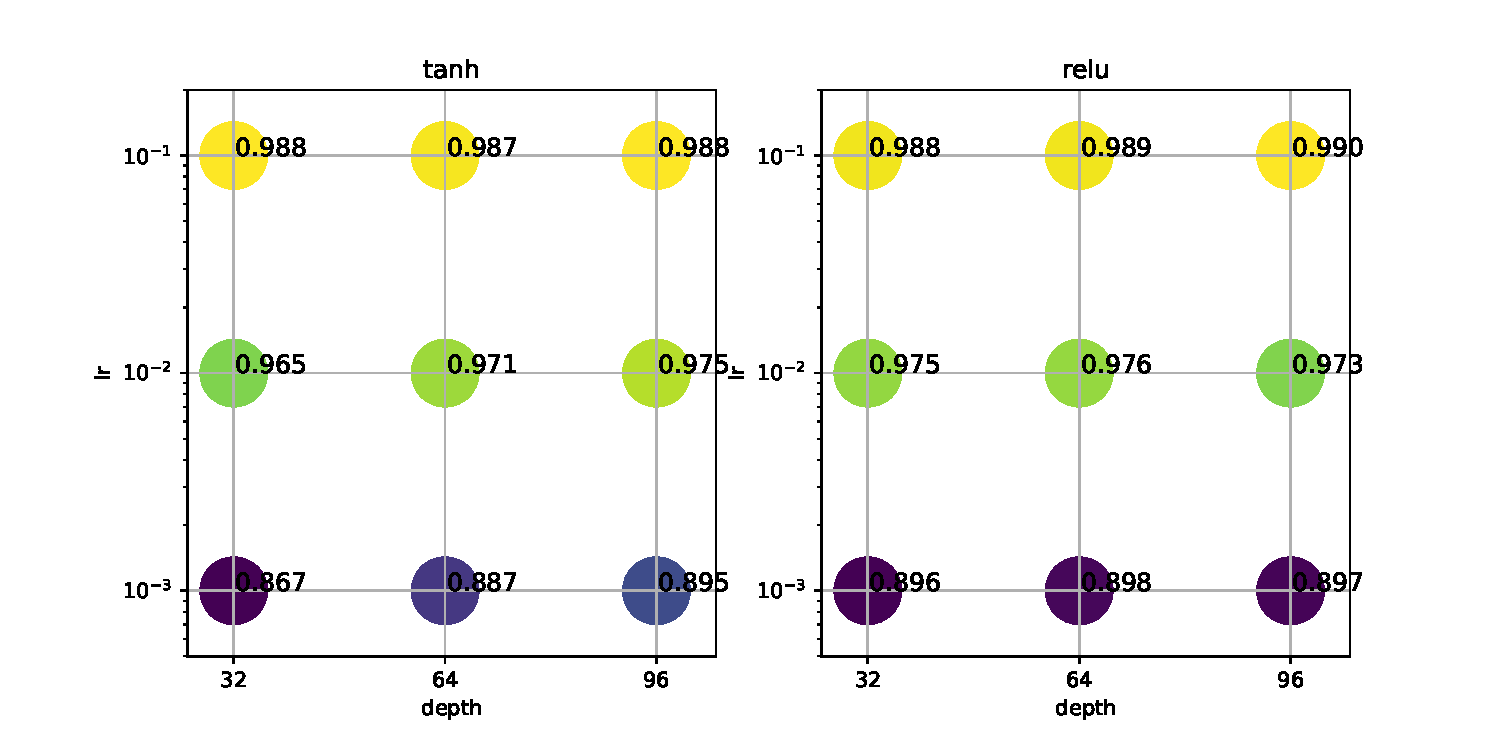
\includegraphics[scale=0.45]{grid_search.pdf}
	\caption{\it Grid search over activation, depth and learning rate.}
	\label{fig:grid}
\end{figure}
\end{frame}

%\begin{frame}
%\frametitle{Grid Search II}
%Check out this picture
%\end{frame}

\begin{frame}
\frametitle{Random Search}
\begin{figure}[t]
	\centering
	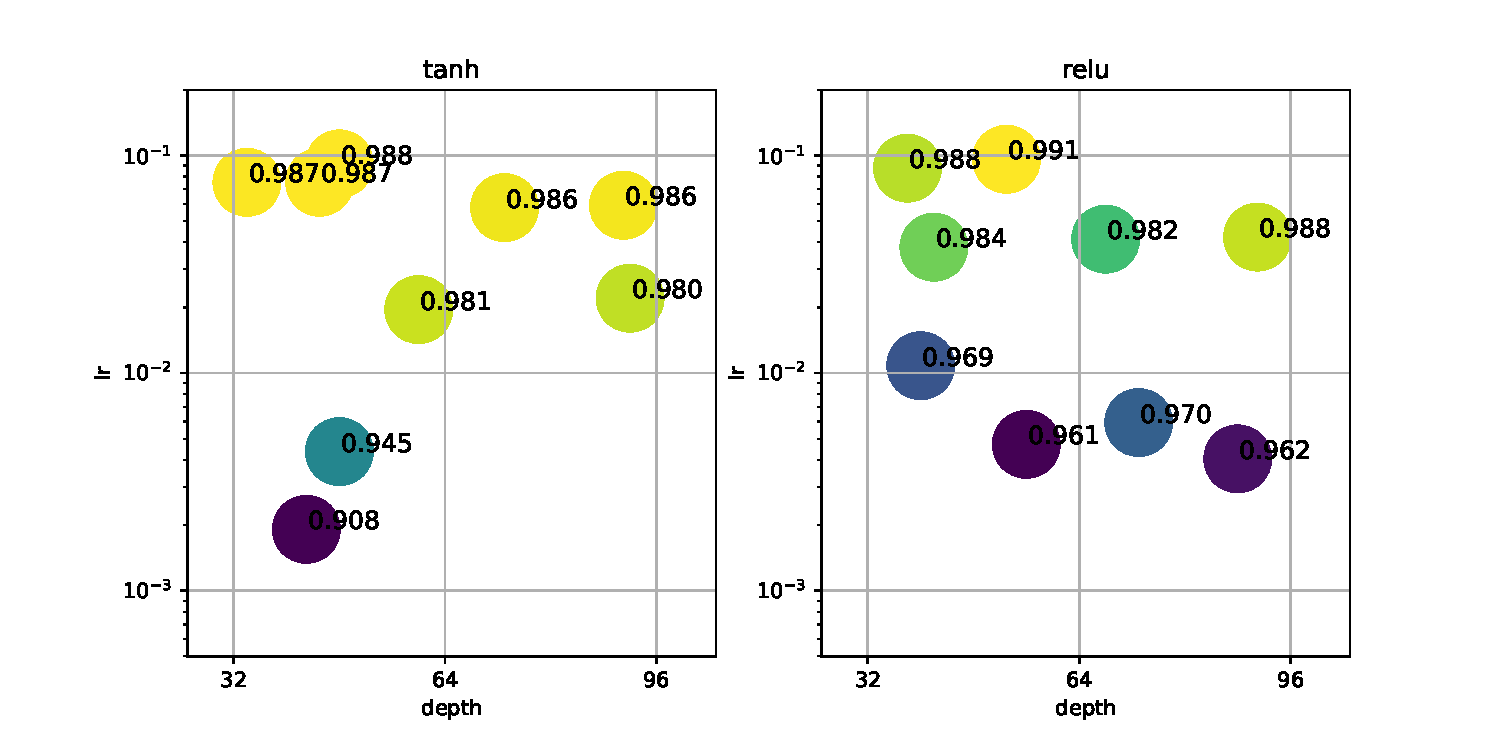
\includegraphics[scale=0.45]{random_search.pdf}
	\caption{\it Random search over activation, depth and learning rate.}
	\label{fig:random}
\end{figure}
\end{frame}

\begin{frame}
\frametitle{Exploration and Exploitation}
Multi armed bandit
\bi
\item Maximize gain with finite number of resources
\item We want to minimize regret
\begin{align}
	\rho = T \cdot \mu^* - \sum_t \hat{r}_t
\end{align}
with $T$ number of round/configurations, $\mu^*$ maximal reward and $\hat{r}_t$ the reward in round $t$.
\item Problem of reinforcement learning
\ei
\pause 
In practice
\bi
\item Many hyperparameters are correlated
\item Should utilize prior knowledge
\ei
\end{frame}

\begin{frame}
\frametitle{Bayesian Optimization}
Utilizing prior results to get better estimates of future configurations.
\bi
\item We model $p(f(\lambda)|D_n)$, where $\lambda \in D_n$ is a data collection of hyperparameters.
\item Use \textbf{acquisitions} function $a: \lambda \rightarrow \mathbb{R}^+$ which trades exploration vs exploitation which will be maximized
\pause
\item Select new parameters: $\lambda_{n+1} = \arg \max_\lambda a(\lambda)$, add new data point $\{f_{n+1}, \lambda_{n+1}\}$ to collection $D_{n+1}$ improve posterior $p(f|D_{n+1})$
\item Common acquisitions function is \textbf{Expected Improvement}
\begin{align}
	a(\lambda_i) = \text{EI}(\lambda_i) = \mathbb{E}_{p(f|D)} [\max( f(\lambda) - f(\lambda^+))]
\end{align}
others are Upper Confident Bound or (Maximum) Probability of Improvement.
\ei
\end{frame}

%some nice notebooks
%https://krasserm.github.io/2018/03/19/gaussian-processes/
%https://krasserm.github.io/2018/03/21/bayesian-optimization/
\begin{frame}
\frametitle{Gaussian optimization}
Gaussian optimization has been shown to consistently outperform random/grid search {\color{blue} [1206.2944]}.
\bi
\item Assume $f$ has some Gaussian process prior given by
\begin{align}
	f \sim \mathcal{GP}(m(\lambda), \Sigma_\theta (\lambda, \lambda') )=  \mathcal{N} (y|m(\lambda), \Sigma_\theta(\lambda, \lambda'))
\end{align}
where $\lambda \in D_n$ and $\Sigma_\theta$ is some covariance matrix% and $\theta$ are further hyperparameters of the Gaussian process.
\item Take for example the following kernel
\begin{align}
	\Sigma_\theta (\lambda_i, \lambda_j) = \theta_1 \exp \left[ - \frac{1}{2 \theta_2} ||\lambda_i - \lambda_j ||^2 \right]
\end{align}
\pause
\item Get posterior $p(f_{n+1}|D_n, \lambda_{n+1}) = \mathcal{N}(y|\mu_n(\lambda_{n+1}), \sigma_n(\lambda_{n+1}))$. Select new parameters according to Expected Improvement with
\begin{align}
	\text{EI}(\lambda) = \begin{cases}
	(\mu(\lambda) - f^+  - \xi) P(\gamma > f^+ ) + \sigma (\lambda) \phi(\gamma)  \\
	0 \qquad \qquad \qquad \qquad \qquad \text{ if } \sigma(\lambda) = 0
	\end{cases}
\end{align}
with $\gamma = \frac{\mu(\lambda) - f^+ - \xi}{\sigma(\lambda)}$ and $\phi(\gamma)$ being the PDF.

\ei
\end{frame}

\begin{frame}
\frametitle{Gaussian in a picture}
\begin{figure}[t]
	\centering
	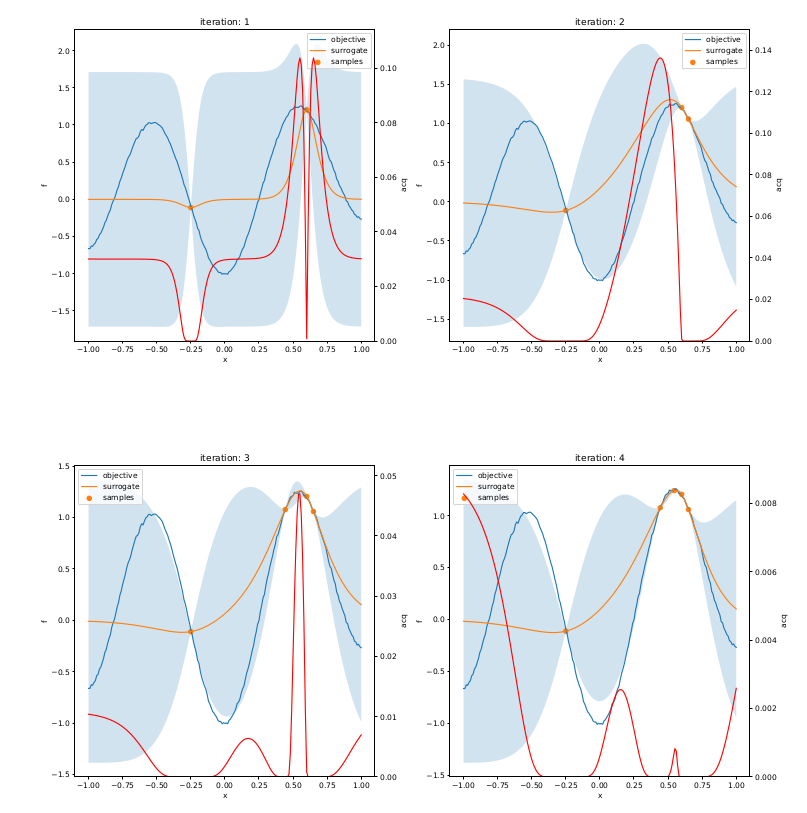
\includegraphics[scale=0.25]{gp_bo.png}
	\caption{\it Gaussian process on 1D problem.}
	\label{fig:bo1d}
\end{figure}
\end{frame}

\begin{frame}
\frametitle{Gaussian in a picture}
\begin{figure}[t]
	\centering
	\includegraphics[scale=0.45]{bo_search.pdf}
	\caption{\it Bayesian optimization with GP over activation, depth and learning rate using {\color{blue}[github.com/fmfn/BayesianOptimization]}.}
	\label{fig:bo}
\end{figure}
\end{frame}

\begin{frame}
\frametitle{General thoughts}

Possible improvements? What to keep in mind? Possible problems? \pause
\bi
\item We do not have an infinite budget. 
\item We might have access to a cluster for parallel distribution.
\item Bad configuration should be stopped early.
\item Simplicity and adaptability.
\ei
\end{frame}

\begin{frame}
\frametitle{Hyperband}
Hyperband: A Novel Bandit-Based Approach to Hyperparameter Optimization {\color{blue}[1603.06560]}.
\bi
\item Solution to infinite-armed bandit in non-stochastic setting and comes within log factors of stochastic setting
\item Improve performance via adaptive resource allocation and early stopping
\item Outperforms standard Bayesian Optimization (up to factor of 30)
\pause
\item Builds up on \textbf{successive halving} with finite budget $B$ and number of test configurations $n$. Example: $B=80, n=16$, then goes through iterations $i.(n_i, r_i)$: $1.(16,1),2.(8,2),3.(4,4),4.(2,8),5.(1,16)$.
\item Two Hyperparameters: $R$ maximum budget to a single computation, $\eta$ controls discarded configurations. Introduce $s_{\max}+1$ with $s_{\max} \approx \log_\eta (R)$ brackets of successive halving. Each bracket uses up to $B$ resources for a total of about $(s_{\max} +1)B$ compute.
\ei
\end{frame}

\begin{frame}
\frametitle{Hyperband II}
\begin{table}
\caption{Hyperband brackets with $\eta = 3$ and budget $R = 81$. On the left we have successive halving with $B = 5 \cdot 81$ and $n = 81$ while to the right $n = 5$.}
	\begin{tabular}{|c|cc|cc|cc|cc|cc|}
	\hline
		& s = & 4 &s =&3 &s =&2 &s =&1 &s =&0 \\
	i &$n_i$ & $r_i$ &$n_i$ & $r_i$ &$n_i$ & $r_i$ &$n_i$ & $r_i$ &$n_i$ & $r_i$ \\
\hline
0 & 81 & 1 & \pause 27 & 3 & \pause 9 & 9 & \pause 6 & 27 & \pause  5 & 81 \\
1 &\pause 27 & 3 & 9 & 9 & 3 & 27 & 2 & 81 && \\
2 & 9 & 9 & 3 & 27 & 1 & 81 & &&& \\
3 & 3 & 27 & 1 & 81 & && &&& \\
4 & 1 & 81 & & & & & &&& \\
\hline
	\end{tabular}
\end{table}
\end{frame}

\begin{frame}
\frametitle{BOHB}
We start from Hyperband, but instead of random picking all the way, we use Bayesian optimization {\color{blue} [1807.01774]}.
\bi
\item Uses Tree Parzen Estimator rather than Gaussian process.
\item Combines the best of both worlds. Fast convergence + better exploitation. 
\item Strong anytime performance.
\item Strong final performance.
\item Tested in various different settings: Kernel methods, deep learning, deep reinforcement learning.
\item Available as a python package.
\ei
\end{frame}

\begin{frame}
\frametitle{BOHB in a picture}
\begin{figure}[t]
	\centering
	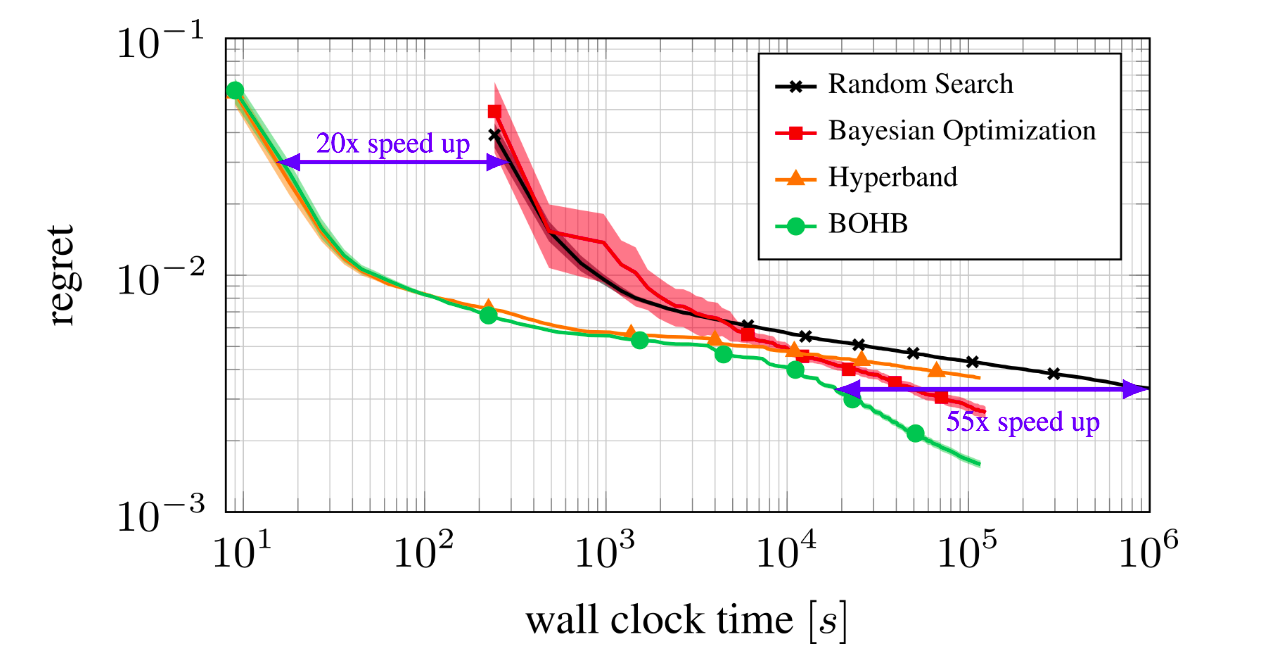
\includegraphics[scale=0.27]{bohb.png}
	\caption{\it BOHB for a neural network over six hyperparameters, taken from {\color{blue} [automl.org/blog\_bohb/]}.}
	\label{fig:bohb}
\end{figure}
\end{frame}

\begin{frame}
\frametitle{Application: Learning CY metrics}
Are there any numerical problems in string theory? Any problems where we do not require 100 \% accuracy? 
\bi
\item We will learn how to construct NNs, which approximate CY metrics.
\item 'Classical' Donaldson algorithm is {\it very} expensive.
\item Dataset: 100.000 points, evaluation of holomorphic volume form and integration weights on Fermat quintic.
\pause
\item There are scalar quantities that measure the deviation from CY metric.
\item Write custom loss and optimize.
\ei
\end{frame}

\begin{frame}
\frametitle{Application: Learning CY metrics}
We have
\begin{align}
	\volcy = \frac{1}{N} \sum_i^N w_i, \qquad \volk = \frac{1}{N} \sum_i^N \frac{\omega^3(p_i)}{\Omega (p_i) \wedge \bar{\Omega} (p_i) } w_i 
\end{align}
\bi
\item Sigma measure
\begin{align}
\sigma  = \frac{1}{N_t \volcy} \sum_{i = 1}^{N_t} \arrowvert 1 - \frac{\omega^3(p_i) / \volk }{ \Omega(p_i) \wedge \bar{\Omega(p_i)} / \volcy} \arrowvert w_i
\end{align}
\item Ricci measure
\begin{align}
|| R ||  = \frac{1}{N_t \volk^{2/3}} \sum_{i = 1}^{N_t}  \frac{\omega^3(p_i) }{ \Omega(p_i) \wedge \bar{\Omega(p_i)} } \lvert R(p_i) \rvert w_i
\end{align}
\ei
\end{frame}


% also check out
%http://neupy.com/2016/12/17/hyperparameter_optimization_for_neural_networks.html#tree-structured-parzen-estimators-tpe
%\begin{frame}
%\frametitle{Tree Parzen Estimator}
%Exists {\color{blue}[github.com/hyperopt/hyperopt]}
%Instead of modeling posterior we model $p(\lambda| y)$ and $p(y)$. Assume for each hyperparameter some prior over some interval $(a,b)$. Then introduce:
%\begin{align}
%p(\lambda| y) = \begin{cases}
%l(\lambda) \text{ if } y < y^* \\
%g(\lambda) \text{ if } y \geq y^*
%\end{cases}
%\end{align}
%where $y^*$ is chosen to be some quantile $\eta$ so that there are points for both distributions.


%Using Bayes theorem we can show that
%\begin{align}
%\text{EI}(\lambda) \propto \left(\eta + \frac{g(\lambda)}{l(\lambda)} (1- \eta) \right)^{-1}
%\end{align}
%Thus want points with high probability $l(\lambda)$ and low $g(\lambda)$.
%\end{frame}

%\begin{frame}
%\frametitle{TPE in a picture}
%\begin{figure}[t]
%\centering
%\includegraphics[scale=0.45]{tpe_search.pdf}
%\caption{\it Bayesian optimization with TPE over activation, depth and learning rate using {\color{blue}[github.com/hyperopt/hyperopt]}.}
%\label{fig:tpe}
%\end{figure}
%\end{frame}


\end{document}